\documentclass{beamer}
\mode<presentation>
\usepackage{amsmath}
\usepackage{amssymb}
%\usepackage{advdate}
\usepackage{adjustbox}
\usepackage{subcaption}
\usepackage{enumitem}
\usepackage{multicol}
\usepackage{mathtools}
\usepackage{listings}
\usepackage{url}
\def\UrlBreaks{\do\/\do-}
\usetheme{Boadilla}
\usecolortheme{lily}
\setbeamertemplate{footline}
{
  \leavevmode%
  \hbox{%
  \begin{beamercolorbox}[wd=\paperwidth,ht=2.25ex,dp=1ex,right]{author in head/foot}%
    \insertframenumber{} / \inserttotalframenumber\hspace*{2ex} 
  \end{beamercolorbox}}%
  \vskip0pt%
}
\setbeamertemplate{navigation symbols}{}

\providecommand{\nCr}[2]{\,^{#1}C_{#2}} % nCr
\providecommand{\nPr}[2]{\,^{#1}P_{#2}} % nPr
\providecommand{\mbf}{\mathbf}
\providecommand{\pr}[1]{\ensuremath{\Pr\left(#1\right)}}
\providecommand{\qfunc}[1]{\ensuremath{Q\left(#1\right)}}
\providecommand{\sbrak}[1]{\ensuremath{{}\left[#1\right]}}
\providecommand{\lsbrak}[1]{\ensuremath{{}\left[#1\right.}}
\providecommand{\rsbrak}[1]{\ensuremath{{}\left.#1\right]}}
\providecommand{\brak}[1]{\ensuremath{\left(#1\right)}}
\providecommand{\lbrak}[1]{\ensuremath{\left(#1\right.}}
\providecommand{\rbrak}[1]{\ensuremath{\left.#1\right)}}
\providecommand{\cbrak}[1]{\ensuremath{\left\{#1\right\}}}
\providecommand{\lcbrak}[1]{\ensuremath{\left\{#1\right.}}
\providecommand{\rcbrak}[1]{\ensuremath{\left.#1\right\}}}
\theoremstyle{remark}
\newtheorem{rem}{Remark}
\newcommand{\sgn}{\mathop{\mathrm{sgn}}}
\providecommand{\abs}[1]{\left\vert#1\right\vert}
\providecommand{\res}[1]{\Res\displaylimits_{#1}} 
\providecommand{\norm}[1]{\lVert#1\rVert}
\providecommand{\mtx}[1]{\mathbf{#1}}
\providecommand{\mean}[1]{E\left[ #1 \right]}
\providecommand{\fourier}{\overset{\mathcal{F}}{ \rightleftharpoons}}
%\providecommand{\hilbert}{\overset{\mathcal{H}}{ \rightleftharpoons}}
\providecommand{\system}{\overset{\mathcal{H}}{ \longleftrightarrow}}
	%\newcommand{\solution}[2]{\textbf{Solution:}{#1}}
%\newcommand{\solution}{\noindent \textbf{Solution: }}
\providecommand{\dec}[2]{\ensuremath{\overset{#1}{\underset{#2}{\gtrless}}}}
\newcommand{\myvec}[1]{\ensuremath{\begin{pmatrix}#1\end{pmatrix}}}
\let\vec\mathbf

\lstset{
%language=C,
frame=single, 
breaklines=true,
columns=fullflexible
}

\numberwithin{equation}{section}

\title{11.16.3.17.1}
\author{Dhawal \\ ee24btech11015,\\IIT Hyderabad.}

\date{\today} 
\begin{document}

\begin{frame}
\titlepage
\end{frame}

\section*{Outline}
\begin{frame}
\tableofcontents
\end{frame}
\section{Problem}
\begin{frame}
\frametitle{Problem Statement}
%
 For an event A, $p\brak{A}=0.42.$ Find $p\brak{A'}$.

\end{frame}

%\subsection{Literature}
\section{Solution}
\subsection{Theoretical Solution}
\begin{frame}
\frametitle{Theoretical Solution}
%\framesubtitle{Literature}
\begin{align}
		p\brak{A'}&=1-p\brak{A}\\
        p\brak{A'}&=0.58
	\end{align}
	

\end{frame}

\subsection{Solution using Bernoulli R.V}
\begin{frame}
\frametitle{Solution using Bernoulli R.V}

The Bernoulli R.V is defined as,
\begin{align}
	X_i = \begin{cases}
		0 & A'\\	
		1 & A	
	\end{cases}
\end{align}

    The PMF represents probability of each outcome in the sample space $S$ . 
\begin{align*}
    S = \sbrak{0, 1},
\end{align*}

The PMF is given as:
\begin{align}
p_X\brak{n} = \begin{cases}
    1-0.42 & n = 0\\
    0.42 & n = 1 \\ 
    0 & n \notin S.
\end{cases}
\end{align}
	

\end{frame}


\subsection{Simulation Process}
\begin{frame}
\frametitle{Simulation Process}

    1) We will define a Bernoulli random variable that generates $1$ for $A$ and $0$ for $A'$.\\
    2) $P\brak{1}=P\brak{A}=0.42$ and $P\brak{0}=P\brak{A'}=0.58$ \\
    3) It will generate 10000 values.\\
    4) Then will find $P\brak{A}$ and $P\brak{A'}$\\
    5) At last we will show stem plot.\\
    Using random function $10000$ times obtain $0$ or $1$, where $p\brak{1}=0.42$ 
\begin{align}
    p\brak{A}=\frac{\text{Number of 1}}{10000}\\
        p\brak{A'}=\frac{\text{Number of 0}}{10000}
\end{align}

\end{frame}


\subsection{Final Solution}
\begin{frame}
\frametitle{Final Solution}
We get,
    \begin{align}
        p\brak{A}=0.4238 \\
        p\brak{A'}=0.5762
    \end{align}
\end{frame}






\section{PLot}
\begin{frame}[fragile]
\frametitle{Plot}

\begin{figure}[h]
    \centering
    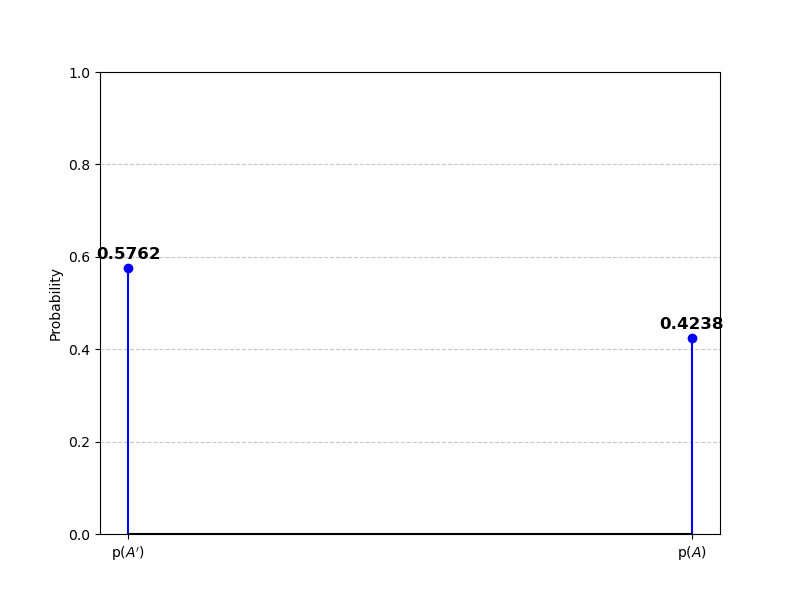
\includegraphics[width=0.9\columnwidth]{figs/Figure_1.png}
    \caption{Plot of the differential equation }
    \label{fig:Plot}
    \end{figure}
\end{frame}

\section{Codes}
\begin{frame}[fragile]
\frametitle{Codes}
\begin{lstlisting}[language=C]
https://github.com/Dhawal24112006/EE1003/tree/main/NCERT/Q7/codes
    \end{lstlisting}
\end{frame}


\end{document}
